\documentclass[12pt, twoside]{article}
\usepackage[letterpaper, margin=1in, headsep=0.5in]{geometry}
\usepackage[english]{babel}
\usepackage[utf8]{inputenc}
\usepackage{amsmath}
\usepackage{amsfonts}
\usepackage{amssymb}
\usepackage{tikz}
\usetikzlibrary{quotes, angles}
\usepackage{graphicx}
%\usepackage{pgfplots}
%\pgfplotsset{width=10cm,compat=1.9}
%\usepgfplotslibrary{statistics}
%\usepackage{pgfplotstable}
%\usepackage{tkz-fct}
%\usepackage{venndiagram}
\usepackage{enumitem}
\usepackage{multicol}


\usepackage{fancyhdr}
\pagestyle{fancy}
\fancyhf{}
\fancyhead[LE]{\thepage}
\fancyhead[RO]{\thepage \\Name: \hspace{4cm} \,\\}
\fancyhead[LO]{BECA / Dr. Huson / Geometry 10th Grade\\* Unit 11: Algebra II introduction \\ 19 April 2020}

\renewcommand{\headrulewidth}{0pt}

\begin{document}
\subsubsection*{11.1 Classwork: Literals, equations with multiple unknowns \\
Do not use a calculator or convert values to decimals}
Reference: Chili Math, Solving Literal Equations \\
https://www.chilimath.com/lessons/intermediate-algebra/literal-equations/

\begin{enumerate}

\subsubsection*{Simplify each expression by ``collecting like terms''}
\item 
\begin{enumerate}[itemsep=2cm]
  \begin{multicols}{2}
    \item $2x+4-x+11$
    \item $5y-4-7y+y$
    \item $14+5\pi-2\pi+4$
    \item $2a+\sqrt{5}+7a+3\sqrt{5}$
    \item $x\sqrt{3}-x\sqrt{3}+x+1$
    \item $3\pi x+4+2 \pi x -7$
  \end{multicols}
  \end{enumerate} \vspace{0.5cm}

\subsubsection*{Solve each equation for the unknown}

One step.
\item 
\begin{enumerate}[itemsep=2cm]
  \begin{multicols}{2}
    \item $2x=12$
    \item $4z=-8$
    \item $3a=\pi$
    \item $2y=\sqrt{5}$
  \end{multicols}
  \end{enumerate} \vspace{1cm}

  Two steps.
\item 
\begin{enumerate}[itemsep=2cm]
  \begin{multicols}{2}
    \item $7x+4=11$
    \item $-4b+5=-3$
    \item $4m-\sqrt{2}=3\sqrt{2}$
    \item $2y-3\pi=\pi$
  \end{multicols}
  \end{enumerate} 

  \newpage

\item   $10=x-3x$ \vspace{3cm}
\item   $\frac{1}{2}(6-2x)=4x$ \vspace{3cm}
\item   $11=\frac{1}{3}x+2x-10$ \vspace{3cm}

\newpage
\subsubsection*{Working with polynomials}
Simplify each expression by ``collecting like terms''
\item 
\begin{enumerate}[itemsep=2cm]
  \begin{multicols}{2}
    \item $4x^2+3x -7 -2x^2-x+4$
    \item $3(a^2-2a +1) -2(a^2-a-4)$
  \end{multicols}
  \end{enumerate} \vspace{1cm}

\subsubsection*{Slope-intercept form}

What is the slope and $y$-intercept of each equation?
\item   $y=2x-3$ \vspace{2cm}
\item   $4x+2y=6$ \vspace{3cm}


\subsubsection*{Function substitution}
\item Given $f(x)=4x+7$. Simplify $f(2)$. \vspace{4cm}
\item Given $\displaystyle f(x)=-\frac{(12+4x)}{11}$. Simplify $f(-3)$.


\newpage
  \item Solve the system of equations by graphing each line and marking the intersection as an ordered pair.
    \[x+y=7\]
    \[y=3x+3\]

\begin{center} %4 quadrant regents grid
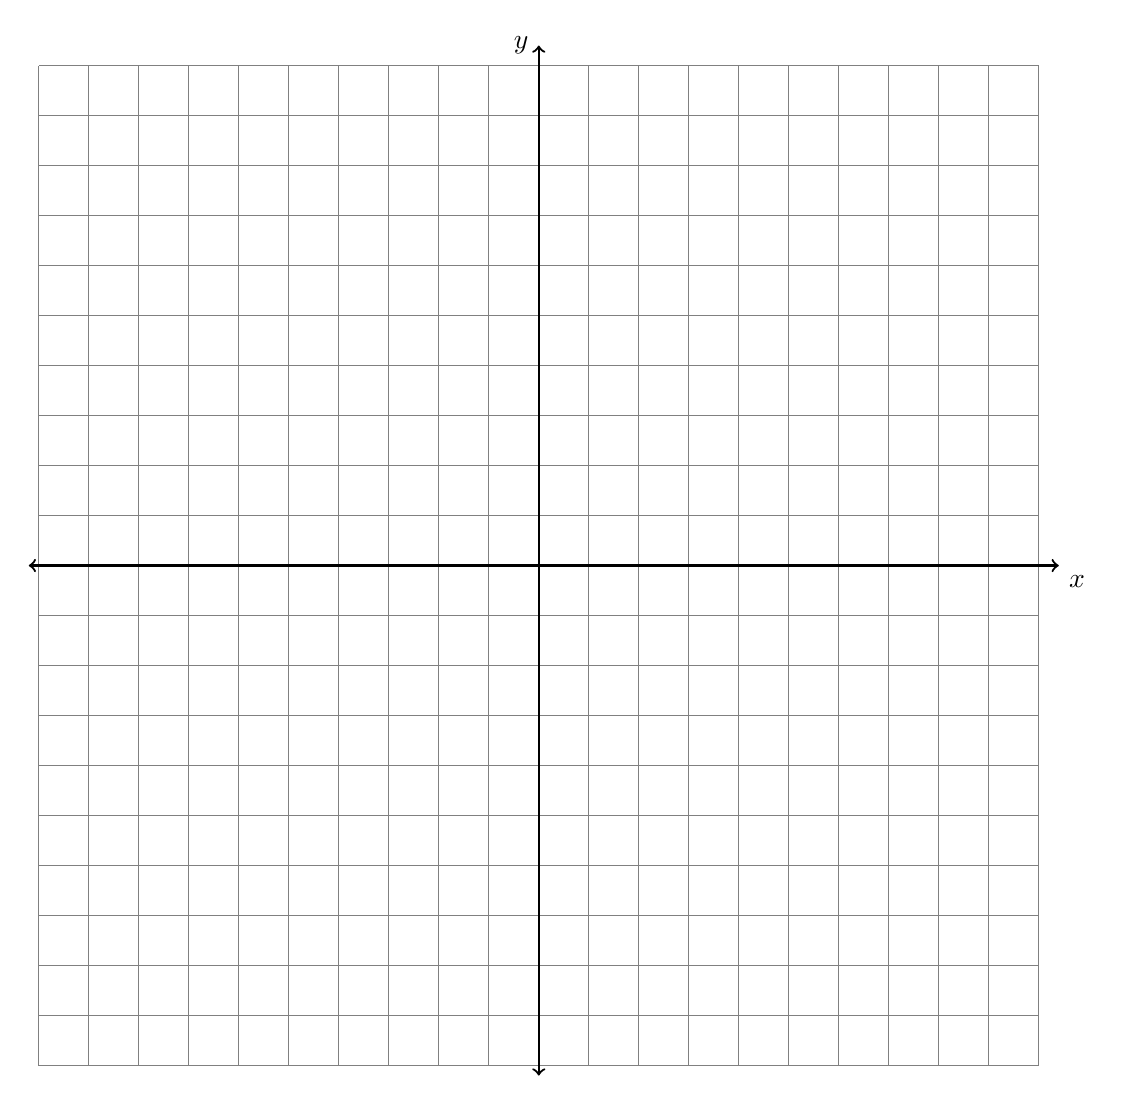
\begin{tikzpicture}[scale=0.635]
  \draw [help lines] (-10,-10) grid (10,10);
  \draw [thick, <->] (-10.2,0) -- (10.4,0) node [below right] {$x$};
  \draw [thick, <->] (0,-10.2)--(0,10.4) node [left] {$y$};
\end{tikzpicture}
\end{center}

\newpage
  Solve each system algebraically.
  \item
  $2x-4y=14$\\*
  $5x+4y=7$ \vspace{6cm}

  \item
  $2x-y=-7$\\*
  $3x+4y=17$  \vspace{6cm}


  

\newpage
  \item Oceanside Bike Rental Shop charges a 17 dollar bike fee plus 6 dollars an hour for renting a bike. Jeffrey paid 53 dollars total. How many hours did he pay to have the bike checked out? \vspace{6cm}

  \item Three friends go bowling. The cost per person per game is \$5.30. The cost to rent shoes is \$2.50 per person. Their total cost is \$55.20. How many games did they play? \vspace{6cm}

  \item The admission fee at a small fair is \$1.50 for children and \$4.00 for adults. On a certain day, 40 people enter the fair and \$85.00 is collected. How many children and how many adults attended?

\newpage
\subsubsection*{Parallel and perpendicular linear equations}

  \item What is the equation of the line with a slope of 2 passing through the point $(0,1)$? \vspace{4cm}
  \item What is the equation of a line parallel to $y=-2x+1$ with a $y$-intercept of 4? \vspace{4cm}
  \item What is the slope of a line perpendicular to the line $x-2y=16$? 
\end{enumerate}
\end{document}

